\documentclass{beamer}
\usepackage[utf8]{inputenc}

\usetheme{Madrid}
\usecolortheme{default}
\usepackage{amsmath,amssymb,amsfonts,amsthm}
\usepackage{txfonts}
\usepackage{tkz-euclide}
\usepackage{listings}
\usepackage{adjustbox}
\usepackage{array}
\usepackage{tabularx}
\usepackage{gvv}
\usepackage{lmodern}
\usepackage{circuitikz}
\usepackage{tikz}
\usepackage{graphicx}

\setbeamertemplate{page number in head/foot}[totalframumber]

\usepackage{tcolorbox}
\tcbuselibrary{minted,breakable,xparse,skins}



\definecolor{bg}{gray}{0.95}
\DeclareTCBListing{mintedbox}{O{}m!O{}}{%
  breakable=true,
  listing engine=minted,
  listing only,
  minted language=#2,
  minted style=default,
  minted options={%
    linenos,
    gobble=0,
    breaklines=true,
    breakafter=,,
    fontsize=\small,
    numbersep=8pt,
    #1},
  boxsep=0pt,
  left skip=0pt,
  right skip=0pt,
  left=25pt,
  right=0pt,
  top=3pt,
  bottom=3pt,
  arc=5pt,
  leftrule=0pt,
  rightrule=0pt,
  bottomrule=2pt,
  toprule=2pt,
  colback=bg,
  colframe=orange!70,
  enhanced,
  overlay={%
    \begin{tcbclipinterior}
    \fill[orange!20!white] (frame.south west) rectangle ([xshift=20pt]frame.north west);
    \end{tcbclipinterior}},
  #3,
}
\lstset{
    language=C,
    basicstyle=\ttfamily\small,
    keywordstyle=\color{blue},
    stringstyle=\color{orange},
    commentstyle=\color{green!60!black},
    numbers=left,
    numberstyle=\tiny\color{gray},
    breaklines=true,
    showstringspaces=false,
}
%------------------------------------------------------------
%This block of code defines the information to appear in the
%Title page
\title %optional
{2.3.5}
\date{September 13,2025}
%\subtitle{A short story}

\author % (optional)
{EE25BTECH11002 - Achat Parth Kalpesh}



\begin{document}

\frame{\titlepage}

\begin{frame}{Question}
Find the angle between the line $\vec{r} = \brak{\hat{i} - \hat{j} + \hat{k}} + \lambda\brak{3\hat{i} - \hat{j} + 2\hat{k}}$ and the plane $\vec{r} \cdot \brak{\hat{i} + \hat{j} + \hat{k}} = 3$.
\end{frame}

\begin{frame}{Theoretical Solution}
Let the direction vector of the line be $\vec{d}$ and the normal vector to the plane be $\vec{n}$.
\begin{align}
    \vec{d} = \begin{myvec}{3\\-1\\2}\end{myvec}   
    \end{align}
    \begin{align}
    \vec{n} = \begin{myvec}{1\\1\\1}\end{myvec}
\end{align}
The angle $\theta$ between a line and a plane is the complement of the angle $\phi$ between the line's direction vector $\vec{d}$ and the plane's normal vector $\vec{n}$.
\end{frame}

\begin{frame}{Equation}
The formula to calculate the angle $\theta$ between the line and the plane is given by:
\begin{align}
\theta = \sin^{-1}\brak{\frac{\abs{\vec{n}^\top\vec{d}}}{\norm{\vec{d}} \norm{\vec{n}}}}
\end{align}

\end{frame}

\begin{frame}{Theoretical Solution}
For the given vectors:
\begin{align}
    \vec{n}^\top\vec{d} &= \brak{3}\brak{1} + \brak{-1}\brak{1} + \brak{2}\brak{1} = 4 \\
    \norm{\vec{d}} &= \sqrt{3^2 + \brak{-1}^2 + 2^2} = \sqrt{14} \\
    \norm{\vec{n}} &= \sqrt{1^2 + 1^2 + 1^2} = \sqrt{3}
\end{align}
Substituting these values into the formula:
\begin{align}
    \theta = \sin^{-1}\brak{\frac{4}{\sqrt{14}\sqrt{3}}} = \frac{4}{\sqrt{42}}
\end{align}
So, the angle $\theta$ is $sin^{-1}\brak{\frac{4}{\sqrt{42}}}$ $\approx$ $37.98\degree$.
\end{frame}

\begin{frame}[fragile]
    \frametitle{C code}
    \begin{lstlisting}
#include <stdio.h>
#include <math.h>
float formula(float *d,float *n)
{
    return asin((d[0]*n[0] + d[1]*n[1] + d[2]*n[2])/(sqrt(d[0]*d[0] + d[1]*d[1] + d[2]*d[2])*sqrt(n[0]*n[0] + n[1]*n[1] + n[2]*n[2])));
}
    \end{lstlisting}
\end{frame}

\begin{frame}[fragile]
    \frametitle{Python Code}
    \begin{lstlisting}[language=Python]
import ctypes
import numpy as np
import matplotlib.pyplot as plt
from mpl_toolkits.mplot3d import Axes3D

# Define the absolute path to the compiled C library.
lib_path = ctypes.CDLL('./f.so')

# Define the argument and return types for the C function
#c_float_p = ctypes.POINTER(ctypes.c_float)
lib_path.formula.argtypes = [
    ctypes.POINTER(ctypes.c_float),
    ctypes.POINTER(ctypes.c_float)
]
lib_path.formula.restype = ctypes.c_float
    \end{lstlisting}
\end{frame}

\begin{frame}[fragile]
    \frametitle{Python Code}
    \begin{lstlisting}[language=Python]
# Prepare the input vectors for problem 2.3.5
d_vec = np.array([3, -1, 2], dtype=np.float32)
n_vec = np.array([1, 1, 1], dtype=np.float32)

#d_p = d_vec.ctypes.data_as(ctypes.POINTER(ctypes.c_float))
#n_p = n_vec.ctypes.data_as(ctypes.POINTER(ctypes.c_float))

# Call the C function to calculate the angle
angle = lib_path.formula(
    d_vec.ctypes.data_as(ctypes.POINTER(ctypes.c_float)),
    n_vec.ctypes.data_as(ctypes.POINTER(ctypes.c_float))
)

print(f"Angle between line and plane: {angle:.4f} degrees")
    \end{lstlisting}
\end{frame}

\begin{frame}[fragile]
    \frametitle{Python Code}
    \begin{lstlisting}[language=Python]
# Plane and Line definitions
a, b, c, d_plane = 1, 1, 1, 3 
line_point = np.array([1, -1, 1])
line_direction = d_vec
intersection_point = line_point + 0.5 * line_direction

# Plotting setup
fig = plt.figure(figsize=(10, 8))
ax = fig.add_subplot(111, projection='3d')
plot_lim = 8

x_plane = np.linspace(-plot_lim, plot_lim, 50)
y_plane = np.linspace(-plot_lim, plot_lim, 50)
X, Y = np.meshgrid(x_plane, y_plane)
Z = (d_plane - a*X - b*Y) / c
Z[(Z > plot_lim) | (Z < -plot_lim)] = np.nan # Masking
    \end{lstlisting}
\end{frame}

\begin{frame}[fragile]
    \frametitle{Python Code}
    \begin{lstlisting}[language=Python]
# Plotting the geometry
ax.plot_surface(X, Y, Z, alpha=0.6, color='cyan')
t = np.linspace(-3, 3, 100)
ax.plot(line_point[0] + t * line_direction[0], 
        line_point[1] + t * line_direction[1], 
        line_point[2] + t * line_direction[2], 
        color='magenta', linewidth=3)
ax.scatter(intersection_point[0], intersection_point[1], intersection_point[2], 
           color='red', s=150, zorder=10)
    \end{lstlisting}
\end{frame}

\begin{frame}[fragile]
    \frametitle{Python Code}
    \begin{lstlisting}[language=Python]

# Formatting the plot
ax.set_xlabel('X-axis'); ax.set_ylabel('Y-axis'); ax.set_zlabel('Z-axis')
ax.set_title('Intersection Plot (Angle calculated in C)', fontsize=16)
ax.set_xlim([-plot_lim, plot_lim]); ax.set_ylim([-plot_lim, plot_lim]); ax.set_zlim([-plot_lim, plot_lim])
ax.set_box_aspect([1,1,1])
plt.grid(True)
plt.legend()

# Save and show the final plot
plt.savefig('plot_from_c_and_python_absolute_path.pdf')
plt.show()
    \end{lstlisting}
\end{frame}

\begin{frame}{Plot}
    \begin{figure}
        \centering
        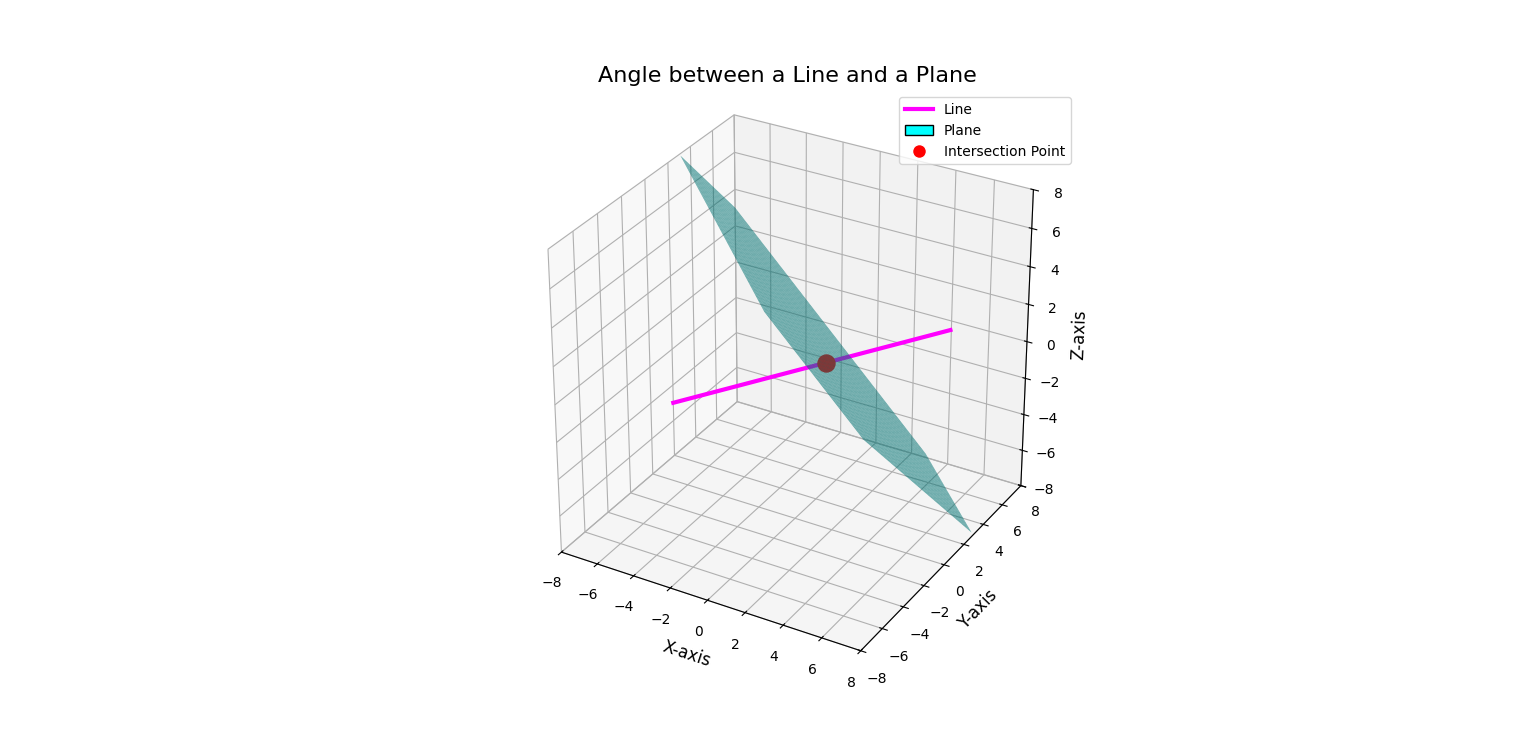
\includegraphics[width=0.7\columnwidth]{../figs/pure_python.png}
        \caption{Angle between the line and plane}
        \label{fig:final_plot}
    \end{figure}
\end{frame}

\end{document}
